\chapter{Theoretical Background}\label{chapter:background} \

In Chapter~\ref{chapter:background} we will introduce the
background information that is required to understand
the main ideas of this thesis. First we introduce
the basic concepts of quantum computing. Then we will
describe advanced concepts regarding quantum noise. We
assume some baseline \ac{ml} knowledge, however, we
will provide an outlook into \ac{qml}. Finally, we
present several types of adversarial machine learning
and adversarial training as a defense mechanism. \

\section{Fundamentals of Quantum Computing} \

% TODO: Most concepts are presented in a simpliflied way.
%       Say most info can be found in books. if not fully
%       understood.

\subsection{Qubit}\label{subsection:qubit} \

The basic computing unit in quantum computing is the
\textit{qubit}~\cite{schumacher_quantum_1995}. Similar to the classical
bit, a qubit also has a state. While a bit has either a
\textit{0} or \textit{1} state, the qubit can have
many more states. The quantum equivalent to the classical
bit states would be \(\ket{0}\) and \(\ket{1}\) in Dirac
notation~\cite{dirac_new_1939} and they represent the orthonormal computational
basis states in Equation~\ref{eq:qubit_bases}. \

\begin{equation}\label{eq:qubit_bases}
    \ket{0} = \begin{pmatrix}
                1 \\ 0
              \end{pmatrix} \qquad \qquad
    \ket{1} = \begin{pmatrix}
                0 \\ 1
              \end{pmatrix}
\end{equation} \

What makes the qubit different and more capable than
the classical bit is that it can also have different states
created by a linear combination or \textit{superposition} from
its basis states. The linear combination in Equation
~\ref{eq:qubit_superposition} is the complete representation
of a qubit, where \(\alpha\) and \(\beta\) are two complex numbers that
are denominated \textit{probability amplitudes}.
The values \(\alpha\) and \(\beta\) represent a distribution, in which
with probability \(|\alpha|^2\) we will observe a \textit{0}
value and with probability \(|\beta|^2\) we will observe a
\textit{1} value. This distribution is determined by the
Born rule~\cite{born_quantenmechanik_1926} and states that \(|\alpha|^2 + |\beta|^2 \stackrel{!}{=} 1\).
The Born rule thus implies that a qubit state is a unitary vector in
a two-dimensional complex vector space. Although the
probability amplitudes can take on any complex value as long
as they fulfill the Born rule, when we perform a measurement
on the qubit it \textit{collapses} to one of the two basis
states. \

\begin{equation}\label{eq:qubit_superposition}
  \ket{\psi} = \alpha\ket{0} + \beta\ket{1}
\end{equation} \

In the real physical world qubits can be implemented by
several different small particles. However, the mathematical
qubit abstraction helps establish a baseline computing unit
for quantum computing independent of which particle it is
being represented by~\cite{nielsen_quantum_2010}. While in this perfect
mathematical description noise does not occur, there are
different mechanisms to represent the noise that quantum
computers suffer from, namely the density operator that will
be introduced in Subsection~\ref{subsection:density_operator}. \

\subsection{Bloch Sphere} \

The qubit state from Equation~\ref{eq:qubit_superposition} can be
rewritten into Equation~\ref{eq:qubit_global_phase}, where \(e\)
is the Euler number, \(i\) is the imaginary number, and \(\gamma\),
\(\varphi\), and \(\theta\) are real numbers. \

\begin{equation}\label{eq:qubit_global_phase}
  \ket{\psi} = e^{i\gamma} \left( \cos{\frac{\theta}{2}}\ket{0} + e^{i\varphi}\sin{\frac{\theta}{2}}\beta\ket{1} \right)
\end{equation} \

Because for a single qubit the global phase \(e^{i\gamma}\) has no
observable effects, we can omit it and write the state of a qubit as: \

\begin{equation}\label{eq:qubit_bloch}
  \ket{\psi} = \cos{\frac{\theta}{2}}\ket{0} + e^{i\varphi}\sin{\frac{\theta}{2}}\beta\ket{1}
\end{equation} \

where \(\theta\) and \(\varphi\) determine a point in the Bloch
sphere~\cite{bloch_nuclear_1946}. The Bloch sphere (Fig.~\ref{fig:bloch_sphere})
is a helpful visual representation for understanding the state of a
qubit. In Section~\ref{section:noise} this representation will be
utilized to show the effects of quantum noise on a quantum state. It
can also be used to visualize the effect of the operations performed
on quantum states, these operations are called \textit{gates} and 
they will be introduced in Subsection~\ref{subsection:gates}. \

\begin{figure}[ht]
  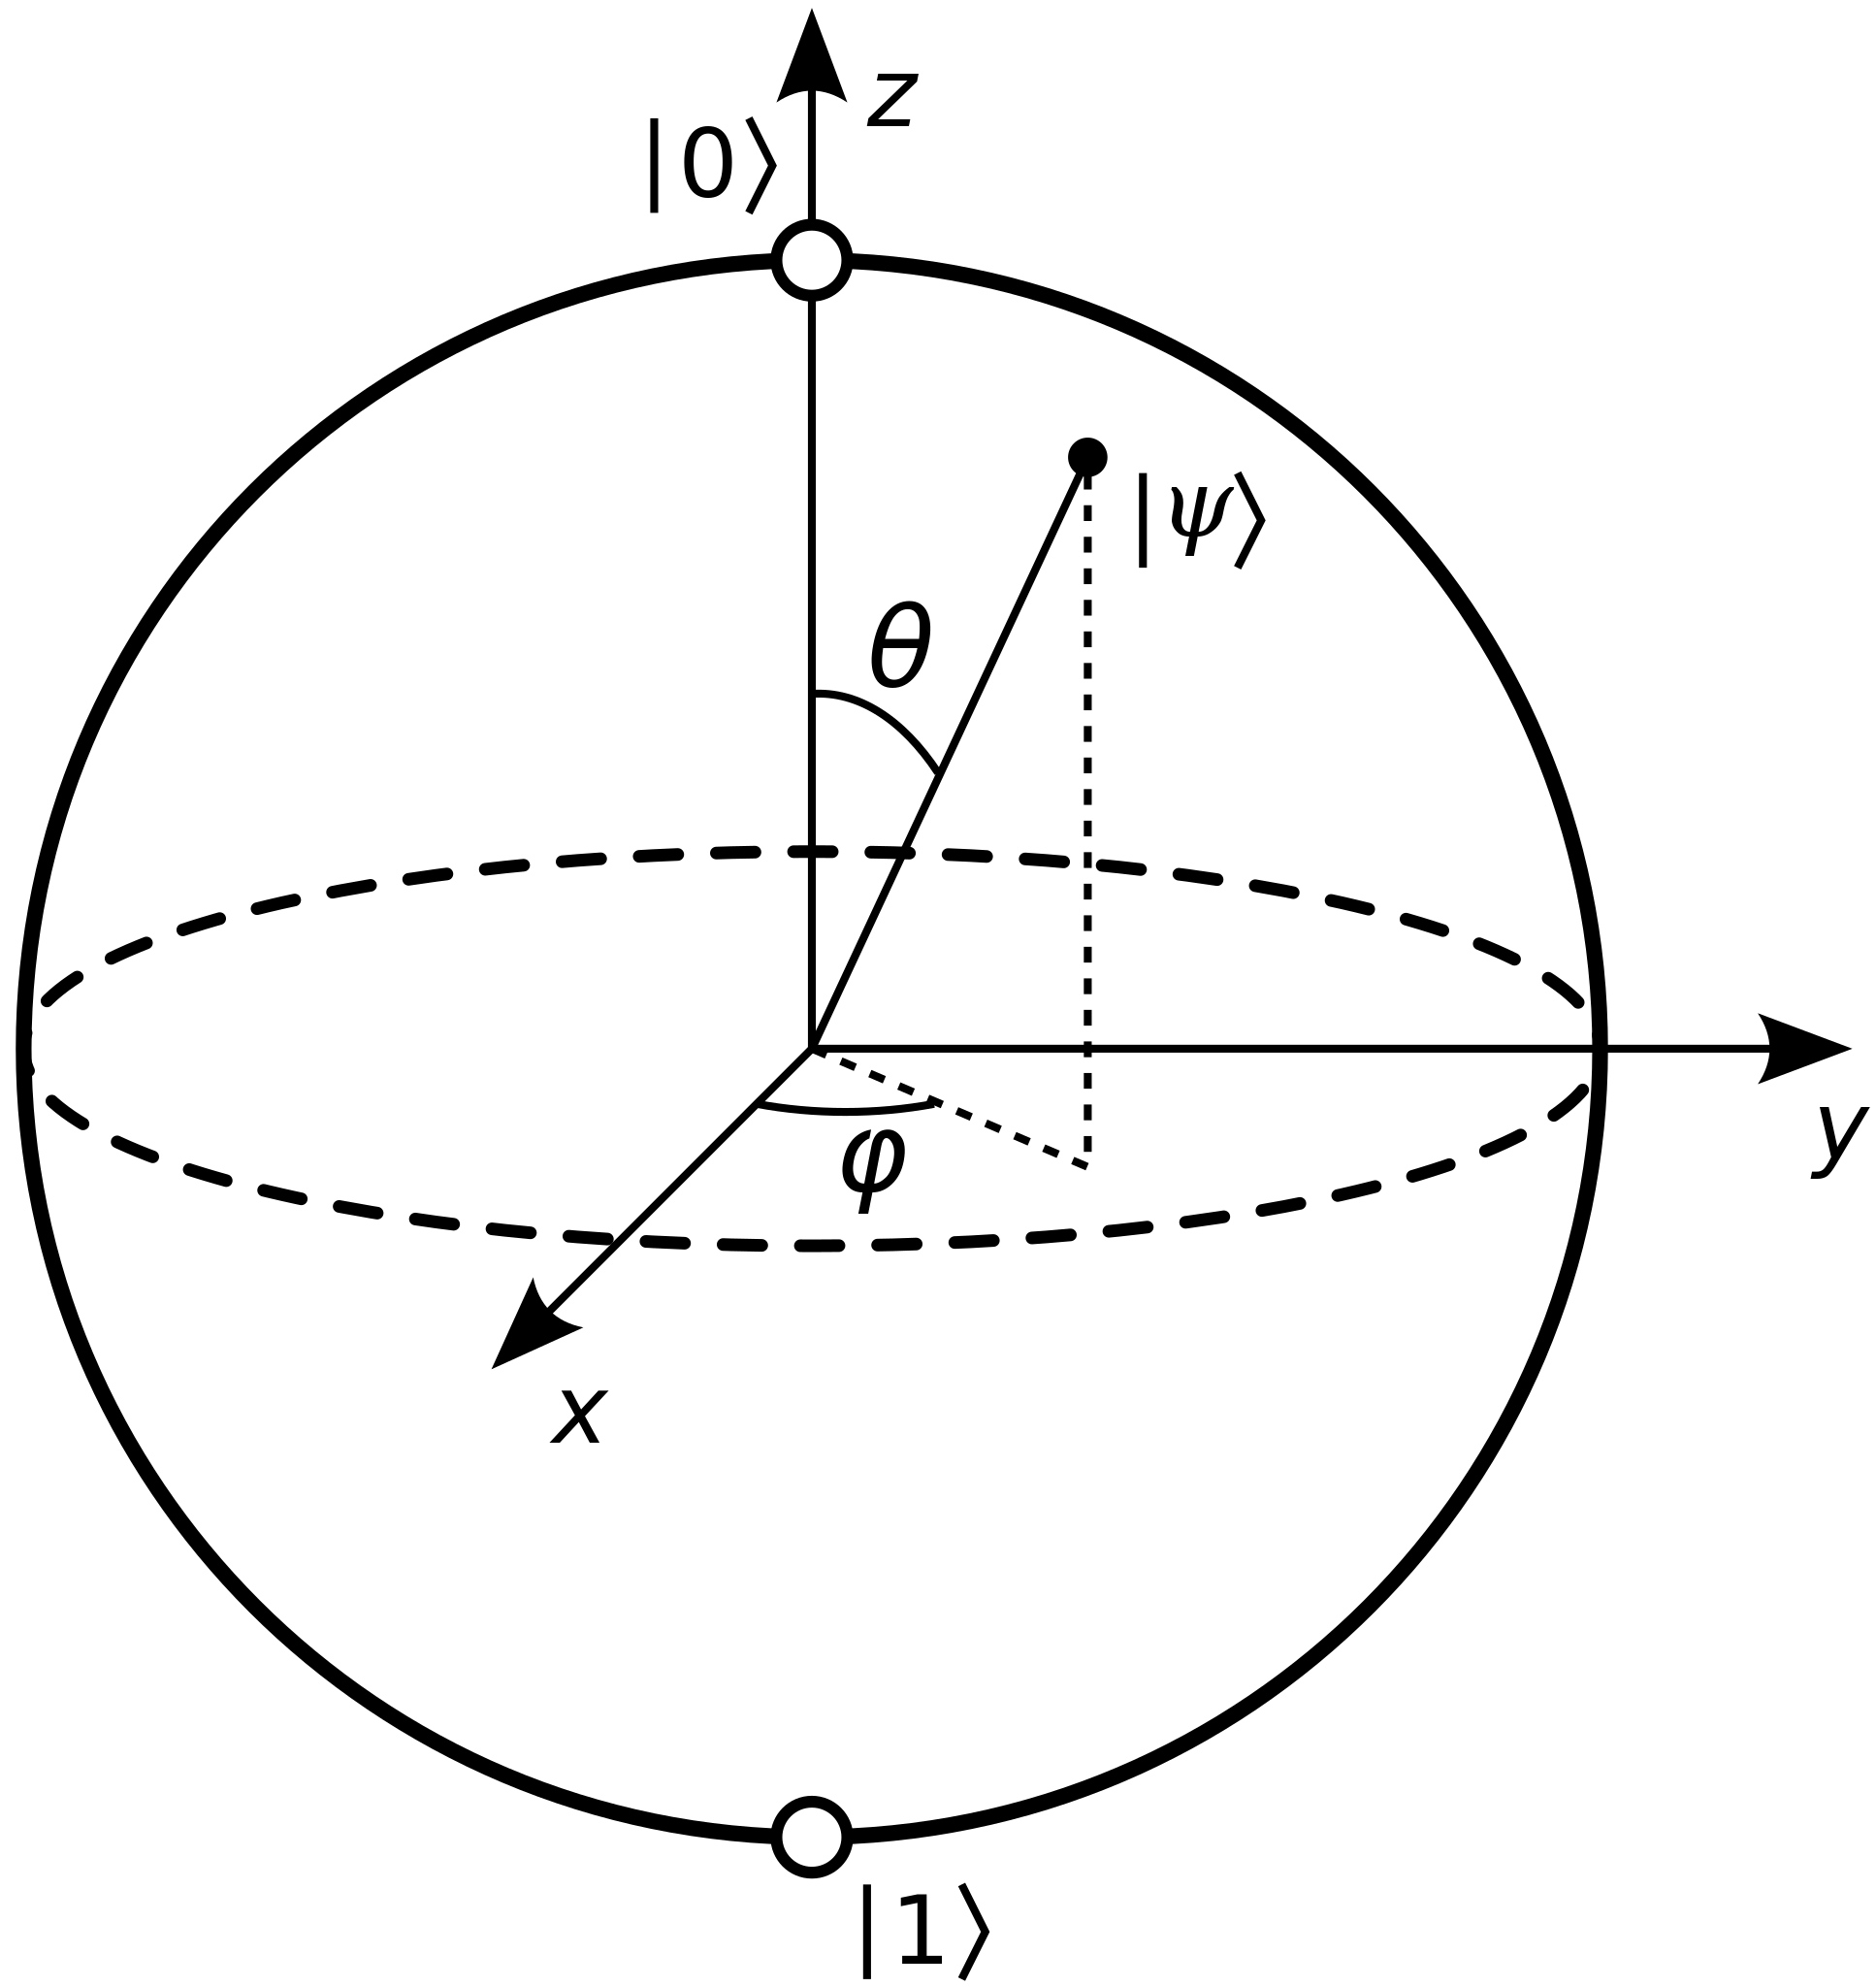
\includegraphics[scale=0.1]{figures/Bloch_sphere.png}
  \centering
  \caption{Bloch sphere representation of a qubit. Image taken from \href{https://commons.wikimedia.org/wiki/File:Bloch_Sphere.svg}{https://commons.wikimedia.org/wiki/File:Bloch\_Sphere.svg} under the \href{https://en.wikipedia.org/wiki/Creative_Commons}{Creative Commons Attribution-Share Alike 3.0 Unported license}.}
~\label{fig:bloch_sphere}
\end{figure} \

\subsection{Multiple qubits} \

To describe multiple qubits we utilize the fundamentals presented in
Subsection~\ref{subsection:qubit} and expand them. For two qubits
\(\ket{00}, \ket{01}, \ket{10}\), and \(\ket{11}\) are the computational basis.
A general representation for a two qubit system can be found in 
Equation~\ref{eq:two_qubits}, where all the probability amplitudes must
follow the Born rule. \ 

\begin{equation}\label{eq:two_qubits}
  \ket{\psi} = \alpha_{00}\ket{00} + \alpha_{01}\ket{01} + \alpha_{10}\ket{10} + \alpha_{11}\ket{11}
\end{equation} \

Due to the Born rule the measurement results for
\(x = \left\{00, 01, 10, 11\right\}\) follow the probability
distribution determined by \(|\alpha_{x}|^2\). Similar to a
single qubit, once a measurement on both qubits is performed,
the state of the qubits will collapse to the measured computational
basis. Nevertheless, with multiple qubits we are able to perform
measurements on a subset of qubits. In the case of a two-qubit
system, measuring the first qubit will collapse its value. However,
the second's qubit state will remain. In the case of Eq.~\ref{eq:two_qubits},
if \textit{0} was measured in the first qubit, the amplitudes \(\alpha_{10}\)
and \(\alpha_{11}\) would disappear from the state as they are no longer
possible. Furthermore, the remaining amplitudes must be normalized,
such as in Eq.~\ref{eq:measure_first}, to fulfill the normalization
restriction.  \

\begin{equation}\label{eq:measure_first}
  \ket{\psi'} = \frac{\alpha_{00}\ket{00} + \alpha_{01}\ket{01}}
                    {\sqrt{|\alpha_{00}|^2 + |\alpha_{01}|^2}}
\end{equation} \

In Equation~\ref*{eq:multiple_qubits} we can find a general representation of
a set of \textit{n} qubits. For a system composed by \textit{n} qubits there are \(2^n\)
amplitudes. If we tried to simulate a quantum system with \(n = 50\), assuming
that complex numbers require 8 bytes to be stored~\cite{numpy}, a classical computer would need
approximately 9000 terabytes to store the generated quantum state. This simple calculation
shows the reason why quantum computers are so promising and also why classical computers
are not able to process quantum information efficiently. \
% (2**50)*8 = 9007199254740992
% https://docs.scipy.org/doc/numpy-1.17.0/user/basics.types.html

\begin{equation}\label{eq:multiple_qubits}
  \ket{\psi} = \alpha_{00}\ket{0\cdots0} + \cdots + \alpha_{2^{n-1}}\ket{1\cdots1}
\end{equation} \

\subsection{Quantum Gates}\label{subsection:gates}\

Once that quantum states have been defined, performing operations
on them is the next step to understand how quantum computing works.
These operations are denominated \textit{quantum gates} and they
modify the quantum state according to its properties. A quantum gate
can be represented as a matrix that fulfills one single property,
namely that it is a unitary matrix. In Equation~\ref{eq:unitary} we
can observe that a unitary matrix is one which when multiplied by its
own transpose conjugate is equal to the identity matrix.

\begin{equation}\label{eq:unitary}
  UU^{\dag} = I
\end{equation}

This property is required because when a quantum gate is used on a
quantum state, the resulting quantum state has to be a valid normalized
quantum state. By being a unitary matrix, this effect is achieved.
There are infinitely many unitary matrices, however, there are some
of specific importance. The most important single-qubit quantum
gates will be introduced in Subsection~\ref{subsubsection:single_qubit},
while the most significant multiple-qubits gates will be presented
in Subsection~\ref{subsubsection:multiple_qubit} \

\subsubsection{Single-Qubit Gates}\label{subsubsection:single_qubit} \

Single-Qubit gates can be described by a two by two unitary matrix. The
first three quantum gates introduced are described by the Pauli matrices.
They are defined as the X, Y and Z gates because each matrix represents
a \(\pi\) rotation around the Bloch sphere in their respective axis. \

\paragraph{X Gate} \

The X gate's matrix and its gate representations can be found in
Equation~\ref{eq:pauli_x}. In classical computing, the X gate is
conceptually equivalent to the NOT gate, thus it
is also known as a quantum NOT gate. \

\begin{equation}\label{eq:pauli_x}
  X = \begin{pmatrix}
        0 & 1 \\
        1 & 0
      \end{pmatrix} \qquad \qquad
  \Qcircuit @C=1em @R=1em {
    & \gate{X} & \qw
  } \qquad
  \Qcircuit @C=1em @R=1em {
    & \targ & \qw
  }
\end{equation} \

In Equation~\ref{eq:pauli_x_basis} we can see the effect of the X
gate, where the computational basis states are flipped. This phenomena
is known as a \textit{bit flip}. \

\begin{equation}\label{eq:pauli_x_basis}
  X\ket{0} = \begin{pmatrix}
               0 & 1 \\
               1 & 0
             \end{pmatrix}
             \begin{pmatrix} 1 \\ 0 \end{pmatrix} = 
             \begin{pmatrix} 0 \\ 1 \end{pmatrix} =
             \ket{1}, \qquad
  X\ket{1} = \begin{pmatrix}
              0 & 1 \\
              1 & 0
            \end{pmatrix}
            \begin{pmatrix} 0 \\ 1 \end{pmatrix} = 
            \begin{pmatrix} 1 \\ 0 \end{pmatrix} =
            \ket{0}
\end{equation} \

\paragraph{Z Gate} \

Unlike the X gate, there is no conceptually equivalent
gate for the Z gate in classical computing. In Equation~\ref{eq:pauli_z}
we can observe the matrix and symbol representation of the Z gate. \

\begin{equation}\label{eq:pauli_z}
  Z = \begin{pmatrix}
        1 & 0 \\
        0 & -1
      \end{pmatrix} \qquad \qquad
  \Qcircuit @C=1em @R=1em {
    & \gate{Z} & \qw
  }
\end{equation} \

The effects of the Z gate can be found in Equation~\ref{eq:pauli_z_basis}.
We can observe that the \(\ket{0}\) state remains unmodified while
the \(\ket{1}\) state is negative after the operation. This phenomena
is known as a \textit{phase flip}. \

\begin{equation}\label{eq:pauli_z_basis}
  Z\ket{0} = \begin{pmatrix}
               1 & 0 \\
               0 & -1
             \end{pmatrix}
             \begin{pmatrix} 1 \\ 0 \end{pmatrix} = 
             \begin{pmatrix} 0 \\ 1 \end{pmatrix} =
             \ket{0}, \qquad
  Z\ket{1} = \begin{pmatrix}
               1 & 0 \\
               0 & -1
            \end{pmatrix}
            \begin{pmatrix} 0 \\ 1 \end{pmatrix} = 
            \begin{pmatrix} 1 \\ 0 \end{pmatrix} =
            -\ket{1}
\end{equation} \

\paragraph{Y Gate} \

The Y gate also doesn't have a conceptually equivalent gate
in classical computing. More interestingly the Y gate can be described
by the product of the X and Z matrix up to a global phase. The matrix
and symbol representation of the Y gate can be found in
Equation~\ref{eq:pauli_y}. \

\begin{equation}\label{eq:pauli_y}
  Y = \begin{pmatrix}
        0 & -i \\
        i & 0
      \end{pmatrix} \qquad \qquad
  \Qcircuit @C=1em @R=1em {
    & \gate{Y} & \qw
  }
\end{equation} \

In Equation~\ref{eq:pauli_y_basis} we can see how the Y gate
modifies the computational basis states. In it we can observe that
a bit flip and a phase flip have been executed, while \(i\) has been
added as a global phase. \

\begin{equation}\label{eq:pauli_y_basis}
  Y\ket{0} = \begin{pmatrix}
               0 & -i \\
               i & 0
             \end{pmatrix}
             \begin{pmatrix} 1 \\ 0 \end{pmatrix} = 
             \begin{pmatrix} 0 \\ 1 \end{pmatrix} =
             i\ket{1}, \qquad
  Y\ket{1} = \begin{pmatrix}
               0 & -i \\
               i & 0
            \end{pmatrix}
            \begin{pmatrix} 0 \\ 1 \end{pmatrix} = 
            \begin{pmatrix} 1 \\ 0 \end{pmatrix} =
            -i\ket{0}
\end{equation} \

As a complement to the Pauli gates, there are gates that
perform a specific \(\theta\) rotation around each axis of the
Bloch sphere. They are known as \(RX\left(\theta\right)\),
\(RY\left(\theta\right)\) and \(RZ\left(\theta\right)\). \

\paragraph{Hadamard Gate} \

The Hadamard gate is one of the most useful single-qubit gates.
It will be later used in Subsection~\ref{subsubsection:entanglement}
to create \textit{entanglement} between two different qubits. \

\begin{equation}\label{eq:hadamard}
  H = \frac{1}{\sqrt{2}} 
      \begin{pmatrix}
        1 & 1 \\
        1 & 1
      \end{pmatrix} \qquad \qquad
  \Qcircuit @C=1em @R=1em {
    & \gate{H} & \qw
  }
\end{equation} \

The effects of the Hadamard gate can be observed in
Equation~\ref{eq:hadamard_basis}. The resulting states from applying
the Hadamard gate to the computational basis are denominated
\(\ket{+}\) and \(\ket{-}\) respectively and they represent
a superposition with equal probability for both basis to be measured. \

\begin{equation}\label{eq:hadamard_basis}
  H\ket{0} = \frac{1}{\sqrt{2}} \left( \ket{0} + \ket{1} \right) = \ket{+} \qquad
  H\ket{1} = \frac{1}{\sqrt{2}} \left( \ket{0} - \ket{1} \right) = \ket{-}
\end{equation} \

Another interesting property of the previously mentioned single-qubit
gates is that all of them are involutory. An involutory matrix is a
square matrix that is its own inverse. This implies that performing
twice the same gate will not modify the quantum state as the identity
transformation would have been applied. \

% MAYBE: Add S and T gates

\subsubsection{Multiple-Qubits Gates}\label{subsubsection:multiple_qubit} \

% TODO: State what the size of the matrix must be depending on the qubits
% it is affecting

\begin{equation}\label{eq:cnot}
  CNOT = \begin{pmatrix}
          1 & 0 & 0 & 0 \\
          0 & 1 & 0 & 0 \\
          0 & 0 & 0 & 1 \\
          0 & 0 & 1 & 0 \\
        \end{pmatrix} \qquad \qquad
  \Qcircuit @C=1em @R=1em {
      & \ctrl{1} & \qw \\
      & \targ & \qw \\
  }
\end{equation} \

\begin{equation}\label{eq:swap}
  SWAP = \begin{pmatrix}
          1 & 0 & 0 & 0 \\
          0 & 0 & 1 & 0 \\
          0 & 1 & 0 & 0 \\
          0 & 0 & 0 & 1 \\
        \end{pmatrix} \qquad \qquad
  \Qcircuit @C=1em @R=1em {
    & \qswap & \qw \\
    & \qswap \qwx & \qw \\
  }
\end{equation} \

% MAYBE: Add toffoli gate

- Introduce quantum circuits \

\subsubsection*{Entanglement}\label{subsubsection:entanglement}

- Introduce entanglement and bell states, 11,16 \
\begin{equation}\label{eq:entanglement}
  \Qcircuit @C=1em @R=1em {
    & \gate{H} & \ctrl{1} & \qw \\
    & \qw & \targ & \qw \\
  } \qquad \qquad
  \frac{1}{\sqrt{2}} \left(\ket{00} + \ket{11}\right)
\end{equation}

- Introduce quantum measurement \
\subsection{Density Operator}\label{subsection:density_operator}
- Introduce the density operator, schuld 87 \
- Introduce quantum algorithms* \

Todo:
- Citation for hadamard gate, pauli gate.

\section{Quantum Noise}\label{section:noise}
i.	Describe the types of noise that can occur.
ii.	Explain where can noise occur.
iii.	State how noise can be simulated.

\section{Quantum Machine Learning}
i.	Present the difference between QML and classical ML\@.
ii.	Introduce variational quantum circuits.
iii.	Explain quantum kernel methods.

\section{Adversarial Machine Learning}
i.	State generalization problems.
ii.	Present different attacks such as FGSM, C\&W, and PGD\@.
iii.	Introduce adversarial training as defence mechanism against adversarial attacks.
iv.	Explain the relationship between general accuracy and adversarial resilience.